\section{User Interface Design}

\subsection{Registration}

% \begin{minipage}{14cm}
%   \centering
%   \begin{minipage}{4.6cm}
%     \centering
%     % \begin{figure}
%       
\includegraphics[width=4.2cm]{inc/ui_reg_step1.jpg}
%     % \end{figure}

%     \raggedright

%     The user presses on the ``create an account'' button when on the app's splash screen.

%   \end{minipage}
%   \begin{minipage}{4.6cm}
%     \centering
%     % \begin{figure}
%       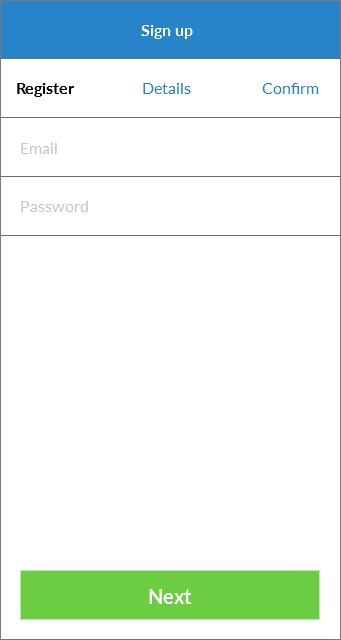
\includegraphics[width=4.2cm]{inc/ui_reg_step2.jpg}
%     % \end{figure}

%     \raggedright

%     The user enters their email address and password. Once done, they press the next button.

%   \end{minipage}
%   \begin{minipage}{4.6cm}
%     \centering
%     % \begin{figure}
%       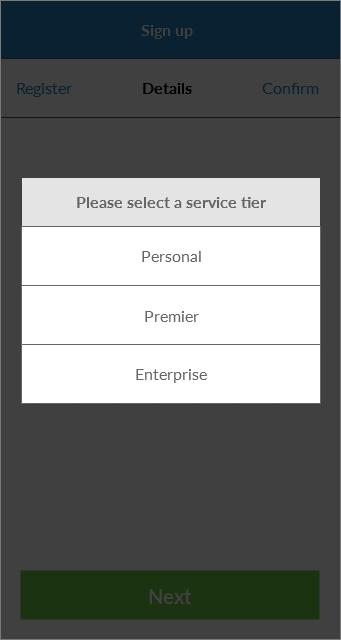
\includegraphics[width=4.2cm]{inc/ui_reg_step3.jpg}
%     % \end{figure}

%     \raggedright

%     The user selects a service tier that is appropriate to their present context.

%   \end{minipage}
% \end{minipage}

\begin{figure}
  \subfigures
  \centering
  \begin{minipage}{4.6cm}
    \centering
    
\includegraphics[width=4.2cm]{inc/ui_reg_step1.jpg}
    \caption{Registration -- Step 1}
    \label{fig:ui_reg_step1}
  \end{minipage}
  \begin{minipage}{4.6cm}
    \centering
    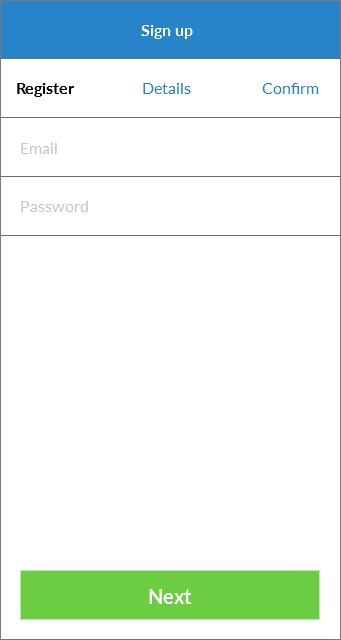
\includegraphics[width=4.2cm]{inc/ui_reg_step2.jpg}
    \caption{Registration -- Step 2}
    \label{fig:ui_reg_step2}
  \end{minipage}
  \begin{minipage}{4.6cm}
    \centering
    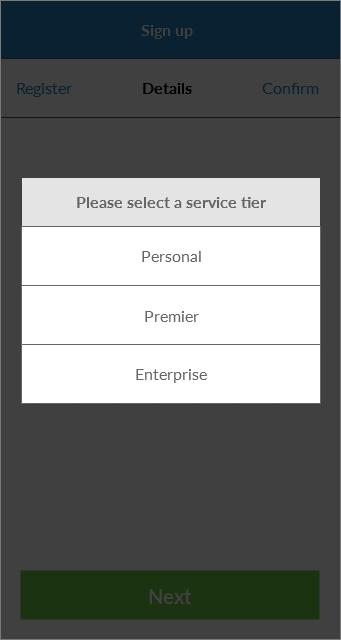
\includegraphics[width=4.2cm]{inc/ui_reg_step3.jpg}
    \caption{Registration -- Step 3}
    \label{fig:ui_reg_step3}
  \end{minipage}
\end{figure}

\begin{minipage}{\textwidth}
  \centering
  \begin{minipage}[t]{4.6cm}
    \vspace{0pt}
    \centering
    \begin{minipage}{4.4cm}
      The user presses on the ``create an account'' button when on the app's splash screen.
    \end{minipage}
  \end{minipage}
  \begin{minipage}[t]{4.6cm}
    \vspace{0pt}
    \centering
    \begin{minipage}{4.4cm}
      The user enters their email address and password. Once done, they press the next button.
    \end{minipage}
  \end{minipage}
  \begin{minipage}[t]{4.6cm}
    \vspace{0pt}
    \centering
    \begin{minipage}{4.4cm}
      The user selects a service tier that is appropriate to their present context.
    \end{minipage}
  \end{minipage}
\end{minipage}

\begin{figure}
  \subfigures
  \centering
  \begin{minipage}{4.6cm}
    \centering
    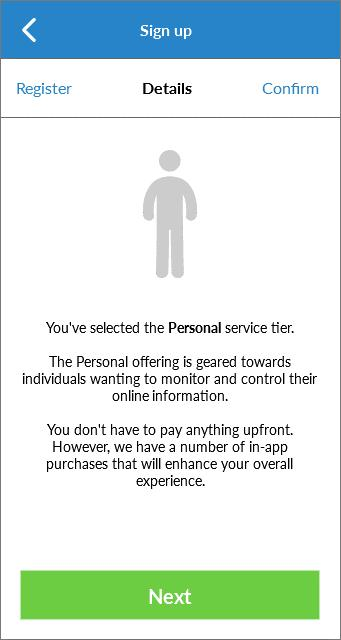
\includegraphics[width=4.2cm]{inc/ui_reg_step4a.jpg}
    \caption{Registration -- Step 4a}
    \label{fig:ui_reg_step4a}
  \end{minipage}
  \begin{minipage}{4.6cm}
    \centering
    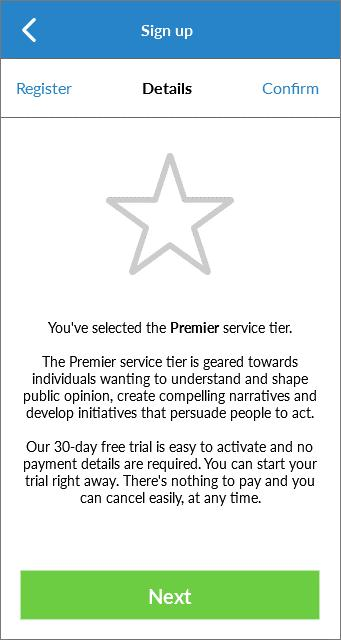
\includegraphics[width=4.2cm]{inc/ui_reg_step4b.jpg}
    \caption{Registration -- Step 4b}
    \label{fig:ui_reg_step4b}
  \end{minipage}
  \begin{minipage}{4.6cm}
    \centering
    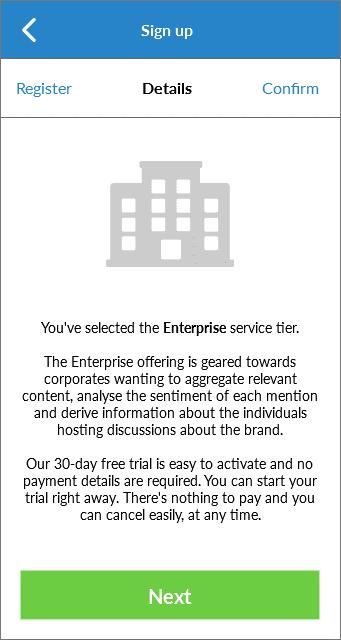
\includegraphics[width=4.2cm]{inc/ui_reg_step4c.jpg}
    \caption{Registration -- Step 4c}
    \label{fig:ui_reg_step4c}
  \end{minipage}
\end{figure}

The user is directed to a screen with details on the selected offering, so that they can be assured of their decision. If they are not, they can press the back button and select another service tier (jump to Register Step 3 see Figure~\ref{fig:ui_reg_step3}). Otherwise, they must press next to carry on.

\begin{figure}
  \centering
  \begin{minipage}{4.6cm}
    \centering
    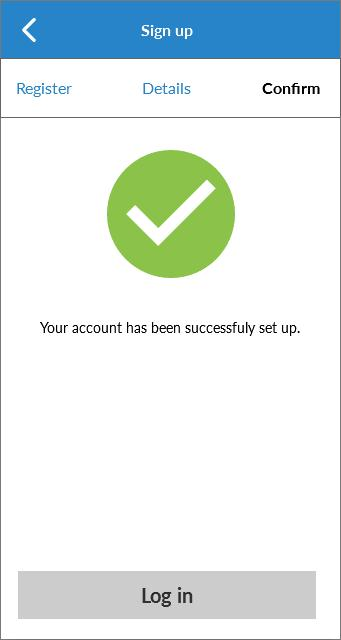
\includegraphics[width=4.2cm]{inc/ui_reg_step5.jpg}
    \caption{Registration -- Step 5}
    \label{fig:ui_step5}
  \end{minipage}
\end{figure}

\begin{minipage}{14cm}
  \centering
  \begin{minipage}{4.4cm}
    Once the account has been set up, the user can sign in step 2 (cf.~\ref{fig:ui_reg_step2}).
  \end{minipage}
\end{minipage}

\subsection{Login}

\begin{figure}
  \subfigures
  \centering
  \begin{minipage}{4.6cm}
    \centering
    
\includegraphics[width=4.2cm]{inc/ui_lg_step1.jpg}
    \caption{Login -- Step 1}
    \label{fig:ui_lg_step1}
  \end{minipage}
  \begin{minipage}{4.6cm}
    \centering
    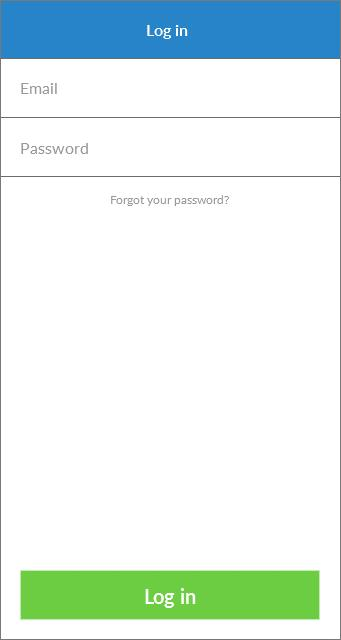
\includegraphics[width=4.2cm]{inc/ui_lg_step2.jpg}
    \caption{Login -- Step 2}
    \label{fig:ui_lg_step2}
  \end{minipage}
  \begin{minipage}{4.6cm}
    \centering
    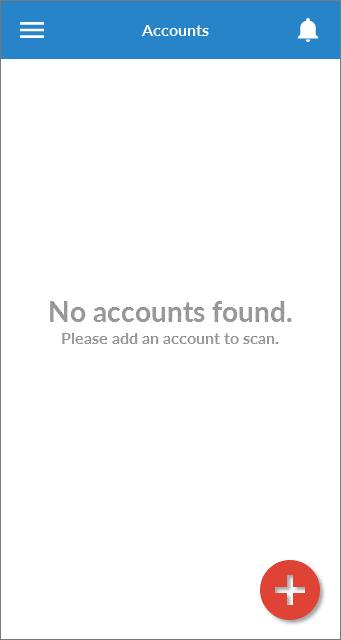
\includegraphics[width=4.2cm]{inc/ui_lg_step3.jpg}
    \caption{Login -- Step 3}
    \label{fig:ui_lg_step3}
  \end{minipage}
\end{figure}

\begin{minipage}{\textwidth}
  \centering
  \begin{minipage}[t]{4.6cm}
    \vspace{0pt}
    \centering
    \begin{minipage}{4.4cm}
      The user presses on the ``already have an account'' text link when on the splash screen.
    \end{minipage}
  \end{minipage}
  \begin{minipage}[t]{4.6cm}
    \vspace{0pt}
    \centering
    \begin{minipage}{4.4cm}
      The user enters their email address and password. Once done, they press the ``log in'' button.
    \end{minipage}
  \end{minipage}
  \begin{minipage}[t]{4.6cm}
    \vspace{0pt}
    \centering
    \begin{minipage}{4.4cm}
      The user is directed to the accounts screen.
    \end{minipage}
  \end{minipage}
\end{minipage}

\subsection{Sidebar Menu}

\begin{figure}
  \subfigures
  \centering
  \begin{minipage}{4.6cm}
    \centering
    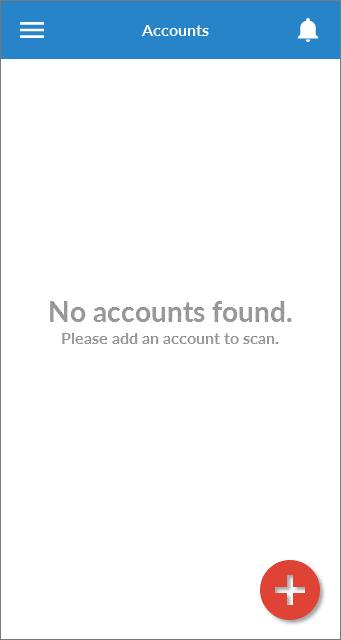
\includegraphics[width=4.2cm]{inc/ui_sb_step1.jpg}
    \caption{View Sidebar Menu -- Step 1}
    \label{fig:ui_sb_step1}
  \end{minipage}
  \begin{minipage}{4.6cm}
    \centering
    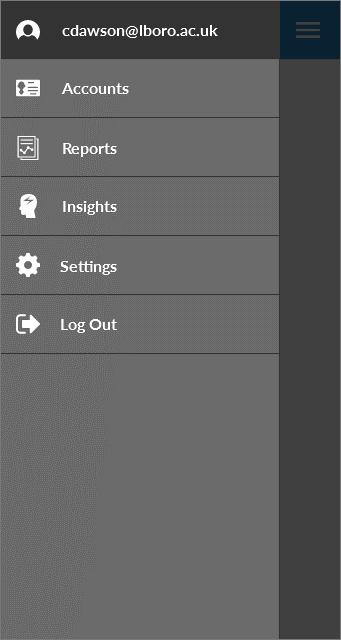
\includegraphics[width=4.2cm]{inc/ui_sb_step2.jpg}
    \caption{View Sidebar Menu -- Step 2}
    \label{fig:ui_sb_step2}
  \end{minipage}
\end{figure}

\begin{minipage}{\textwidth}
  \centering
  \begin{minipage}[t]{4.6cm}
    \vspace{0pt}
    \centering
    \begin{minipage}{4.4cm}
      The user presses on the hamburger icon located in the top left corner.
    \end{minipage}
  \end{minipage}
  \begin{minipage}[t]{4.6cm}
    \vspace{0pt}
    \centering
    \begin{minipage}{4.4cm}
      The sidebar menu slides out from the left, and the user can switch to a different part of the app.
    \end{minipage}
  \end{minipage}
\end{minipage}

\clearpage

\subsection{Notifications}

\begin{figure}
  \subfigures
  \centering
  \begin{minipage}{4.6cm}
    \centering
    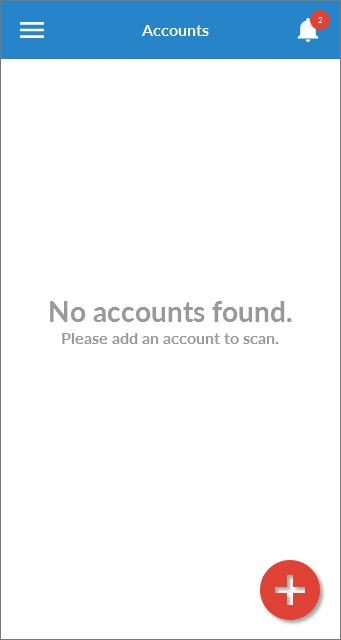
\includegraphics[width=4.2cm]{inc/ui_not_step1.jpg}
    \caption{Notifications -- Step 1}
    \label{fig:ui_not_step1}
  \end{minipage}
  \begin{minipage}{4.6cm}
    \centering
    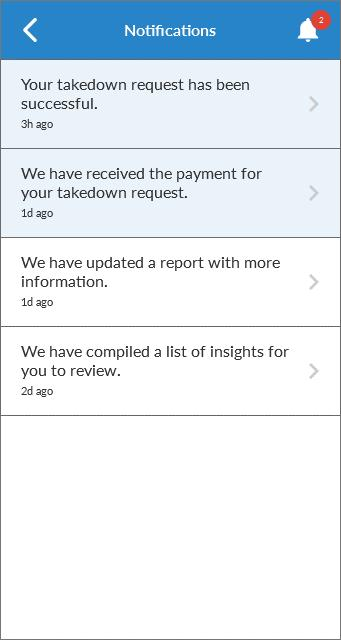
\includegraphics[width=4.2cm]{inc/ui_not_step2.jpg}
    \caption{Notifications -- Step 2}
    \label{fig:ui_not_step2}
  \end{minipage}
  \begin{minipage}{4.6cm}
    \centering
    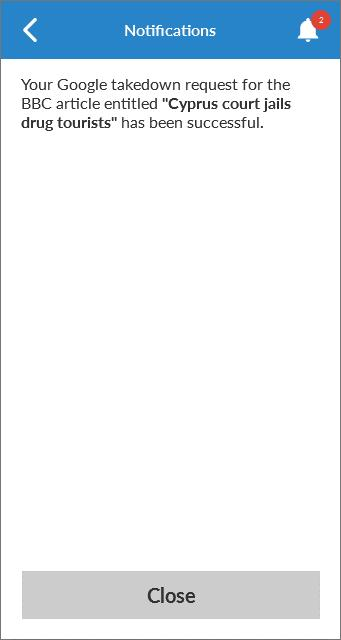
\includegraphics[width=4.2cm]{inc/ui_not_step3.jpg}
    \caption{Notifications -- Step 3}
    \label{fig:ui_not_step3}
  \end{minipage}
\end{figure}

\begin{minipage}{\textwidth}
  \centering
  \begin{minipage}[t]{4.6cm}
    \vspace{0pt}
    \centering
    \begin{minipage}{4.4cm}
      The user presses on the bell icon located in the top right corner whenever they have notifications.
    \end{minipage}
  \end{minipage}
  \begin{minipage}[t]{4.6cm}
    \vspace{0pt}
    \centering
    \begin{minipage}{4.4cm}
      The user is presented with a list of notifications. Items in light blue have not yet been viewed.
    \end{minipage}
  \end{minipage}
  \begin{minipage}[t]{4.6cm}
    \vspace{0pt}
    \centering
    \begin{minipage}{4.4cm}
      Once the user presses on a notification item, more information on the item is displayed.
    \end{minipage}
  \end{minipage}
\end{minipage}

\clearpage

\subsection{Add Account}

\begin{figure}
  \subfigures
  \centering
  \begin{minipage}{4.6cm}
    \centering
    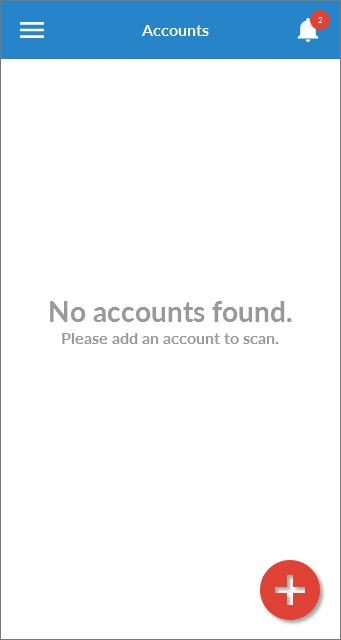
\includegraphics[width=4.2cm]{inc/ui_addacc_step1.jpg}
    \caption{Add Account -- Step 1}
    \label{fig:ui_addacc_step1}
  \end{minipage}
  \begin{minipage}{4.6cm}
    \centering
    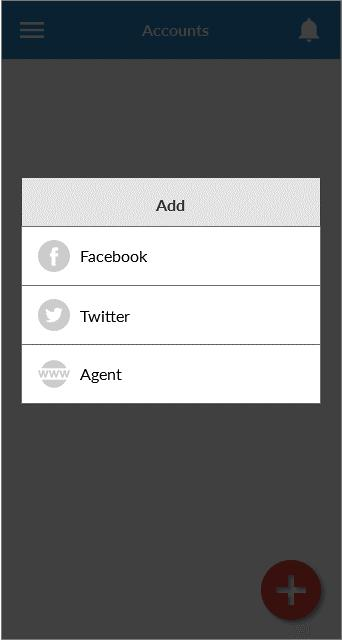
\includegraphics[width=4.2cm]{inc/ui_addacc_step2.jpg}
    \caption{Add Account -- Step 2}
    \label{fig:ui_addacc_step2}
  \end{minipage}
  \begin{minipage}{4.6cm}
    \centering
    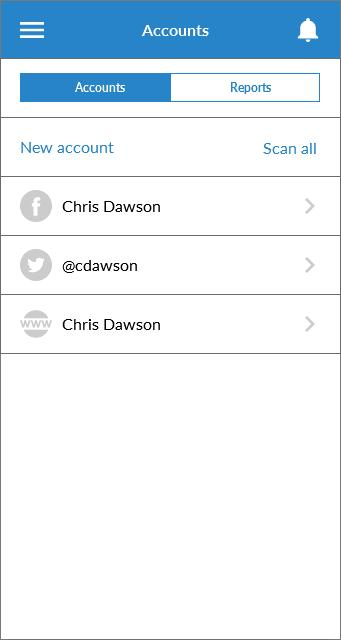
\includegraphics[width=4.2cm]{inc/ui_addacc_step3.jpg}
    \caption{Add Account -- Step 3}
    \label{fig:ui_addacc_step3}
  \end{minipage}
\end{figure}

\begin{minipage}{\textwidth}
  \centering
  \begin{minipage}[t]{4.6cm}
    \vspace{0pt}
    \centering
    \begin{minipage}{4.4cm}
      The user presses on the plus icon located in the bottom right corner to set up a new account.
    \end{minipage}
  \end{minipage}
  \begin{minipage}[t]{4.6cm}
    \vspace{0pt}
    \centering
    \begin{minipage}{4.4cm}
      The user is then presented with a list of account types which can be added to the app.
    \end{minipage}
  \end{minipage}
  \begin{minipage}[t]{4.6cm}
    \vspace{0pt}
    \centering
    \begin{minipage}{4.4cm}
      Once the account has been added, it appears as a persistent entry on the accounts screen.
    \end{minipage}
  \end{minipage}
\end{minipage}

\clearpage

\subsection{Scan Account}

\begin{figure}
  \subfigures
  \centering
  \begin{minipage}{4.6cm}
    \centering
    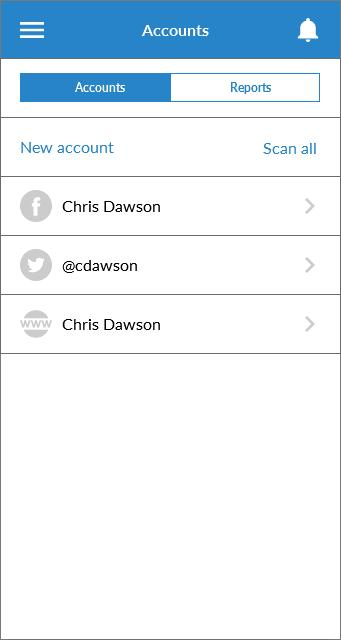
\includegraphics[width=4.2cm]{inc/ui_scan_step1.jpg}
    \caption{Scan Account -- Step 1}
    \label{fig:ui_scan_step1}
  \end{minipage}
  \begin{minipage}{4.6cm}
    \centering
    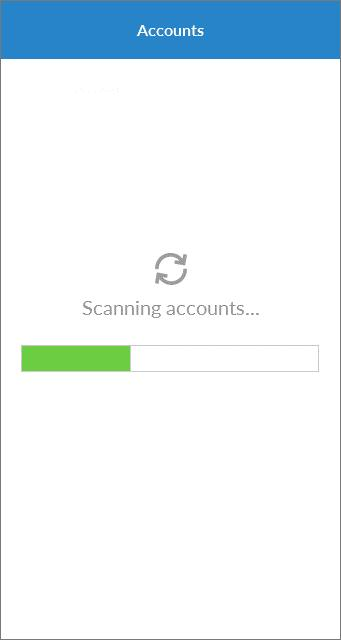
\includegraphics[width=4.2cm]{inc/ui_scan_step2.jpg}
    \caption{Scan Account -- Step 2}
    \label{fig:ui_scan_step2}
  \end{minipage}
  \begin{minipage}{4.6cm}
    \centering
    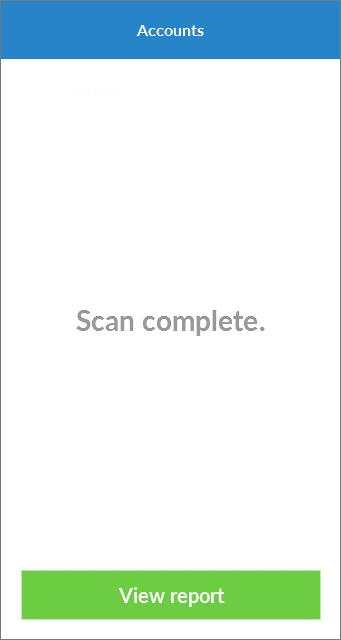
\includegraphics[width=4.2cm]{inc/ui_scan_step3.jpg}
    \caption{Scan Account -- Step 3}
    \label{fig:ui_scan_step3}
  \end{minipage}
\end{figure}

\begin{minipage}{\textwidth}
  \centering
  \begin{minipage}[t]{4.6cm}
    \vspace{0pt}
    \centering
    \begin{minipage}{4.4cm}
      In order to start a scan across all accounts, the user presses on the ``scan all'' link.
    \end{minipage}
  \end{minipage}
  \begin{minipage}[t]{4.6cm}
    \vspace{0pt}
    \centering
    \begin{minipage}{4.4cm}
      The app then scans all accounts in the background, leaving the user to carry on doing other things.
    \end{minipage}
  \end{minipage}
  \begin{minipage}[t]{4.6cm}
    \vspace{0pt}
    \centering
    \begin{minipage}{4.4cm}
      Once a scan is completed, a report summarising the user's current online profile is generated.
    \end{minipage}
  \end{minipage}
\end{minipage}

\clearpage

\subsection{View Accounts}

\begin{figure}
  \subfigures
  \centering
  \begin{minipage}{4.6cm}
    \centering
    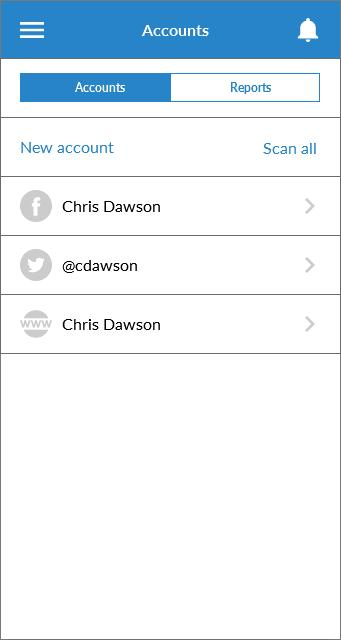
\includegraphics[width=4.2cm]{inc/ui_view_step1.jpg}
    \caption{View Accounts -- Step 1}
    \label{fig:ui_view_step1}
  \end{minipage}
  \begin{minipage}{4.6cm}
    \centering
    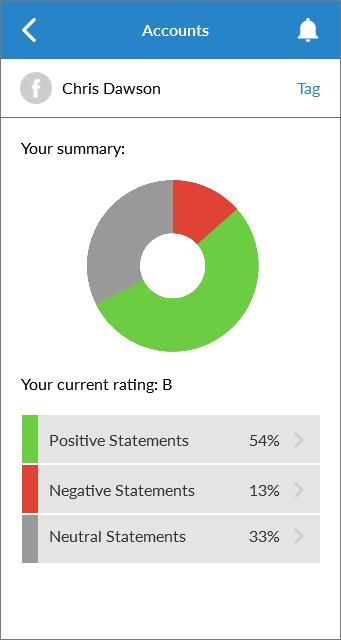
\includegraphics[width=4.2cm]{inc/ui_view_step2.jpg}
    \caption{View Accounts -- Step 2}
    \label{fig:ui_view_step2}
  \end{minipage}
  \begin{minipage}{4.6cm}
    \centering
    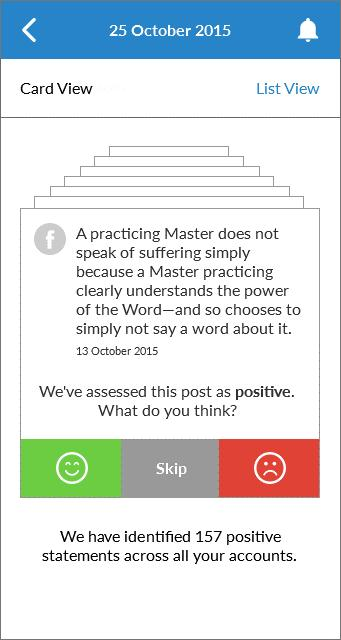
\includegraphics[width=4.2cm]{inc/ui_view_step3.jpg}
    \caption{View Accounts -- Step 3}
    \label{fig:ui_view_step3}
  \end{minipage}
\end{figure}

\begin{minipage}{\textwidth}
  \centering
  \begin{minipage}[t]{4.6cm}
    \vspace{0pt}
    \centering
    \begin{minipage}{4.4cm}
      Once a scan is run across all accounts, the user can view the current status of single accounts.
    \end{minipage}
  \end{minipage}
  \begin{minipage}[t]{4.6cm}
    \vspace{0pt}
    \centering
    \begin{minipage}{4.4cm}
      After the user selects an account, they are presented with a breakdown of its current status.
    \end{minipage}
  \end{minipage}
  \begin{minipage}[t]{4.6cm}
    \vspace{0pt}
    \centering
    \begin{minipage}{4.4cm}
      The user can then assess whether the app has grouped each statement correctly.
    \end{minipage}
  \end{minipage}
\end{minipage}

\clearpage

\subsection{Add Text Tag}

\begin{figure}
  \subfigures
  \centering
  \begin{minipage}{4.6cm}
    \centering
    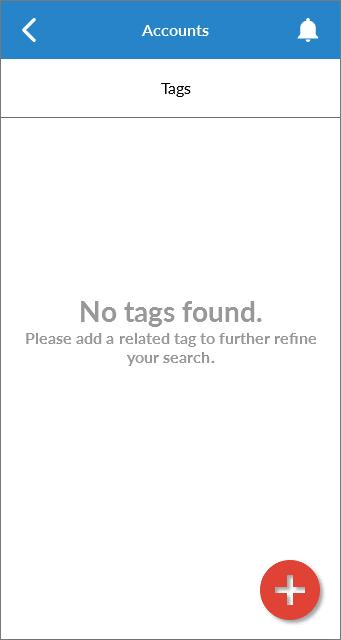
\includegraphics[width=4.2cm]{inc/ui_tag_step1.jpg}
    \caption{Add Text Tag -- Step 1}
    \label{fig:ui_tag_step1}
  \end{minipage}
  \begin{minipage}{4.6cm}
    \centering
    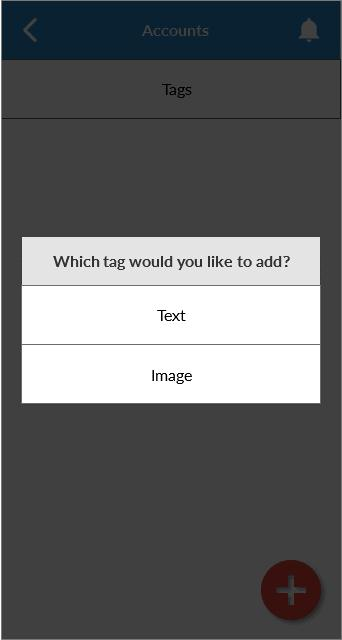
\includegraphics[width=4.2cm]{inc/ui_tag_step2.jpg}
    \caption{Add Text Tag -- Step 2}
    \label{fig:ui_tag_step2}
  \end{minipage}
  \begin{minipage}{4.6cm}
    \centering
    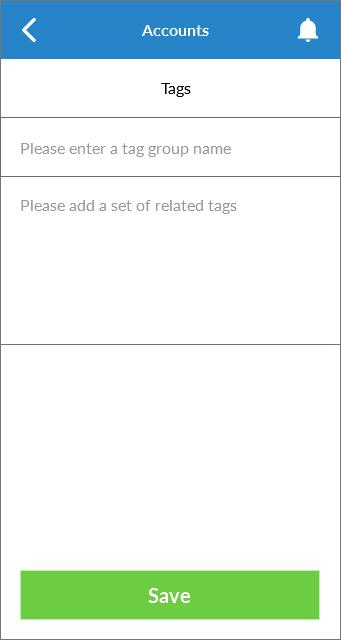
\includegraphics[width=4.2cm]{inc/ui_tag_step3.jpg}
    \caption{Add Text Tag -- Step 3}
    \label{fig:ui_tag_step3}
  \end{minipage}
\end{figure}

\begin{minipage}{\textwidth}
  \centering
  \begin{minipage}[t]{4.6cm}
    \vspace{0pt}
    \centering
    \begin{minipage}{4.4cm}
      Agent accounts are web scrapers that trawl the web and return any requested data to the user.
    \end{minipage}
  \end{minipage}
  \begin{minipage}[t]{4.6cm}
    \vspace{0pt}
    \centering
    \begin{minipage}{4.4cm}
      Text tags can be added to agent accounts in order to refine the quality of results gathered.
    \end{minipage}
  \end{minipage}
  \begin{minipage}[t]{4.6cm}
    \vspace{0pt}
    \centering
    \begin{minipage}{4.4cm}
      Each tag must be assigned a group name and related words (e.g. bio $\rightarrow$ Chris, Loughborough).
    \end{minipage}
  \end{minipage}
\end{minipage}

\clearpage

\subsection{Add Image Tag}

\begin{figure}
  \subfigures
  \centering
  \begin{minipage}{4.6cm}
    \centering
    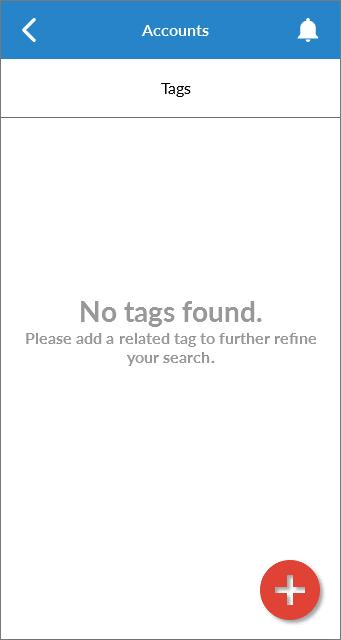
\includegraphics[width=4.2cm]{inc/ui_itag_step1.jpg}
    \caption{Add Image Tag -- Step 1}
    \label{fig:ui_itag_step1}
  \end{minipage}
  \begin{minipage}{4.6cm}
    \centering
    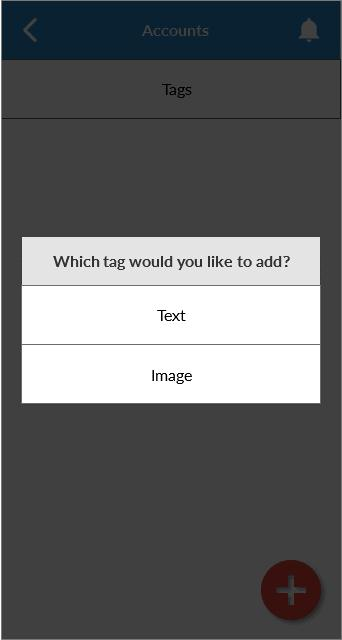
\includegraphics[width=4.2cm]{inc/ui_itag_step2.jpg}
    \caption{Add Image Tag -- Step 2}
    \label{fig:ui_itag_step2}
  \end{minipage}
  \begin{minipage}{4.6cm}
    \centering
    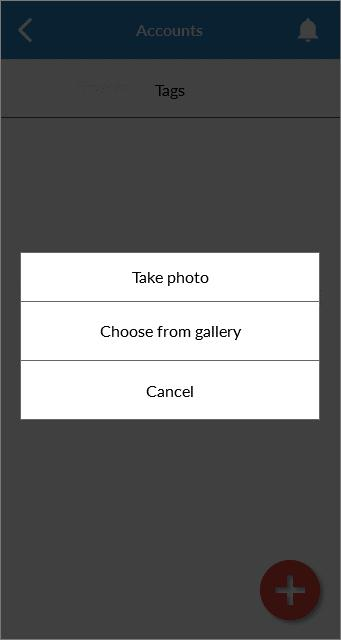
\includegraphics[width=4.2cm]{inc/ui_itag_step3.jpg}
    \caption{Add Image Tag -- Step 3}
    \label{fig:ui_itag_step3}
  \end{minipage}
\end{figure}

\begin{minipage}{\textwidth}
  \centering
  \begin{minipage}[t]{4.6cm}
    \vspace{0pt}
    \centering
    \begin{minipage}{4.4cm}
      The user presses on the plus icon located in the bottom right corner to set up a new tag.
    \end{minipage}
  \end{minipage}
  \begin{minipage}[t]{4.6cm}
    \vspace{0pt}
    \centering
    \begin{minipage}{4.4cm}
      Image tags can be used whenever the user wants to detect any occurrences of copyright abuse.
    \end{minipage}
  \end{minipage}
  \begin{minipage}[t]{4.6cm}
    \vspace{0pt}
    \centering
    \begin{minipage}{4.4cm}
      The user can either select to take a new photo or select one from their phone’s gallery.
    \end{minipage}
  \end{minipage}
\end{minipage}

\begin{figure}
  \subfigures
  \centering
  \begin{minipage}{4.6cm}
    \centering
    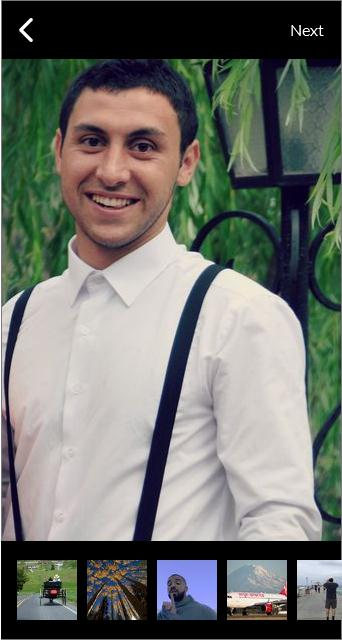
\includegraphics[width=4.2cm]{inc/ui_itag_step4.jpg}
    \caption{Add Image Tag -- Step 4}
    \label{fig:ui_itag_step4}
  \end{minipage}
  \begin{minipage}{4.6cm}
    \centering
    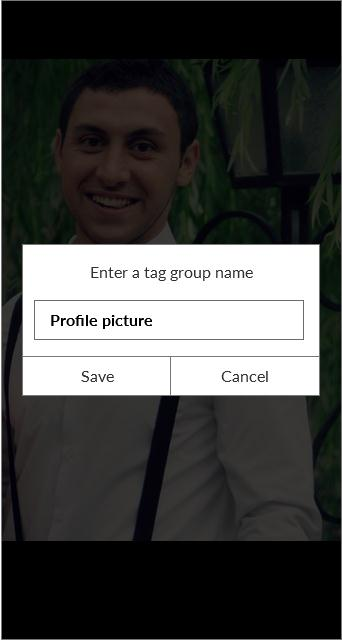
\includegraphics[width=4.2cm]{inc/ui_itag_step5.jpg}
    \caption{Add Image Tag -- Step 5}
    \label{fig:ui_itag_step5}
  \end{minipage}
  \begin{minipage}{4.6cm}
    \centering
    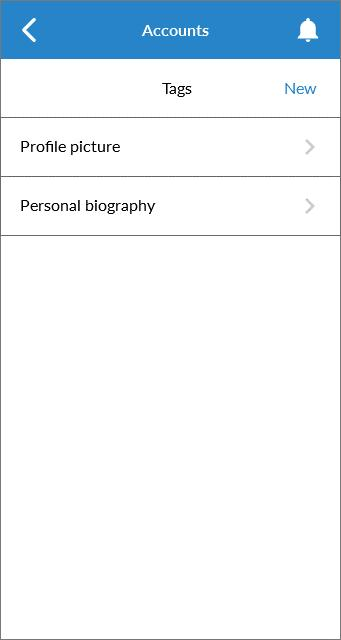
\includegraphics[width=4.2cm]{inc/ui_itag_step6.jpg}
    \caption{Add Image Tag -- Step 6}
    \label{fig:ui_itag_step6}
  \end{minipage}
\end{figure}

\begin{minipage}{\textwidth}
  \centering
  \begin{minipage}[t]{4.6cm}
    \vspace{0pt}
    \centering
    \begin{minipage}{4.4cm}
      In this case, the user has opted to select a profile shot from their phone's gallery for upload.
    \end{minipage}
  \end{minipage}
  \begin{minipage}[t]{4.6cm}
    \vspace{0pt}
    \centering
    \begin{minipage}{4.4cm}
      The user must specify a tag group for the image. Multiple images can be added to one tag group.
    \end{minipage}
  \end{minipage}
  \begin{minipage}[t]{4.6cm}
    \vspace{0pt}
    \centering
    \begin{minipage}{4.4cm}
      Once image and text tags are added, they appear as an entry on the corresponding agent's screen.
    \end{minipage}
  \end{minipage}
\end{minipage}

\subsection{Create Report}

\begin{figure}
  \subfigures
  \centering
  \begin{minipage}{4.6cm}
    \centering
    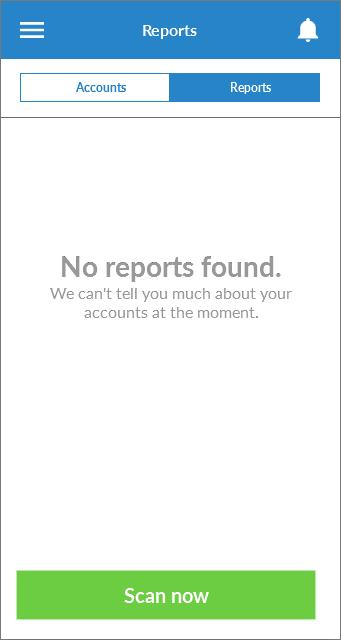
\includegraphics[width=4.2cm]{inc/ui_create_report_step1.jpg}
    \caption{Create Report -- Step 1}
    \label{fig:ui_create_report_step1}
  \end{minipage}
  \begin{minipage}{4.6cm}
    \centering
    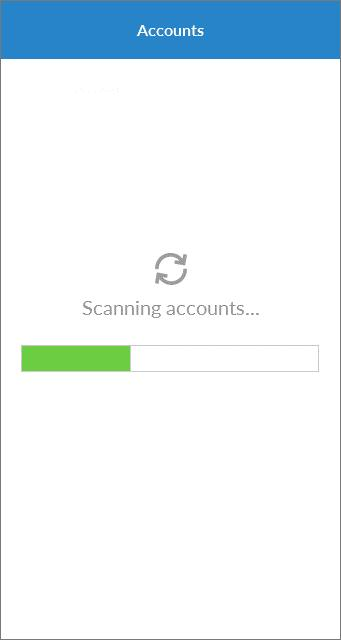
\includegraphics[width=4.2cm]{inc/ui_create_report_step2.jpg}
    \caption{Create Report -- Step 2}
    \label{fig:ui_create_report_step2}
  \end{minipage}
  \begin{minipage}{4.6cm}
    \centering
    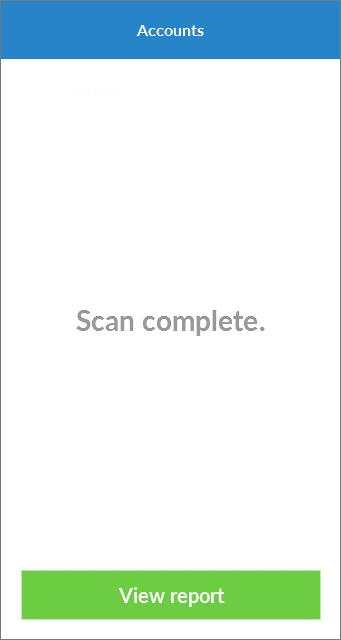
\includegraphics[width=4.2cm]{inc/ui_create_report_step3.jpg}
    \caption{Create Report -- Step 3}
    \label{fig:ui_create_report_step3}
  \end{minipage}
\end{figure}

\begin{minipage}{\textwidth}
  \centering
  \begin{minipage}[t]{4.6cm}
    \vspace{0pt}
    \centering
    \begin{minipage}{4.4cm}
      In order to create a new report for all accounts, the user must press on the ``scan now'' button.
    \end{minipage}
  \end{minipage}
  \begin{minipage}[t]{4.6cm}
    \vspace{0pt}
    \centering
    \begin{minipage}{4.4cm}
      After pressing the ``scan now'' button, a new report is compiled for the user in the background.
    \end{minipage}
  \end{minipage}
  \begin{minipage}[t]{4.6cm}
    \vspace{0pt}
    \centering
    \begin{minipage}{4.4cm}
      Once a scan is completed, a report summarising the user's current online profile is generated.
    \end{minipage}
  \end{minipage}
\end{minipage}

\clearpage

\subsection{View Reports (Card Mode)}

\begin{figure}
  \subfigures
  \centering
  \begin{minipage}{4.6cm}
    \centering
    
\includegraphics[width=4.2cm]{inc/ui_report_card_mode_step1.jpg}
    \caption{View Reports (Card Mode) -- Step 1}
    \label{fig:ui_report_card_mode_step1}
  \end{minipage}
  \begin{minipage}{4.6cm}
    \centering
    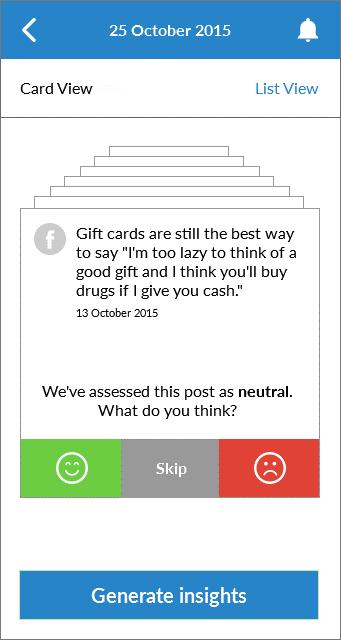
\includegraphics[width=4.2cm]{inc/ui_report_card_mode_step2.jpg}
    \caption{View Reports (Card Mode) -- Step 2}
    \label{fig:ui_report_card_mode_step2}
  \end{minipage}
\end{figure}

\begin{minipage}{\textwidth}
  \centering
  \begin{minipage}[t]{4.6cm}
    \vspace{0pt}
    \centering
    \begin{minipage}{4.4cm}
      After a scan is completed, a new report item appears as an entry on the accounts screen.
    \end{minipage}
  \end{minipage}
  \begin{minipage}[t]{4.6cm}
    \vspace{0pt}
    \centering
    \begin{minipage}{4.4cm}
      Once a report is selected, the user must go through each post to assess if it was grouped correctly.
    \end{minipage}
  \end{minipage}
\end{minipage}

\clearpage

\subsection{View Reports (List Mode)}

\begin{figure}
  \subfigures
  \centering
  \begin{minipage}{4.6cm}
    \centering
    
\includegraphics[width=4.2cm]{inc/ui_report_list_mode_step1.jpg}
    \caption{View Reports (List Mode) -- Step 1}
    \label{fig:ui_report_list_mode_step1}
  \end{minipage}
  \begin{minipage}{4.6cm}
    \centering
    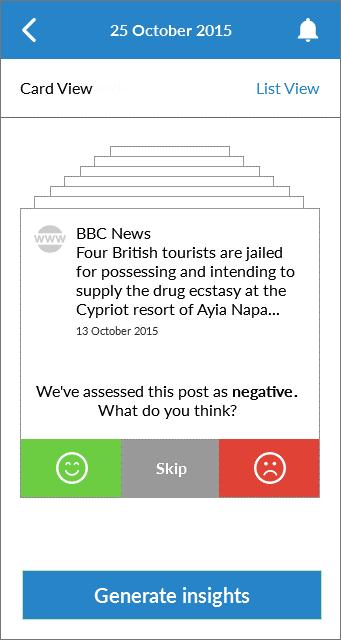
\includegraphics[width=4.2cm]{inc/ui_report_list_mode_step2.jpg}
    \caption{View Reports (List Mode) -- Step 2}
    \label{fig:ui_report_list_mode_step2}
  \end{minipage}
  \begin{minipage}{4.6cm}
    \centering
    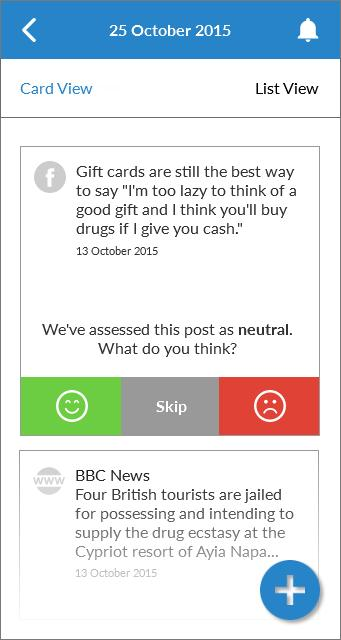
\includegraphics[width=4.2cm]{inc/ui_report_list_mode_step3.jpg}
    \caption{View Reports (List Mode) -- Step 3}
    \label{fig:ui_report_list_mode_step3}
  \end{minipage}
\end{figure}

\begin{minipage}{\textwidth}
  \centering
  \begin{minipage}[t]{4.6cm}
    \vspace{0pt}
    \centering
    \begin{minipage}{4.4cm}
      After a scan is completed, a new report item appears as an entry on the accounts screen.
    \end{minipage}
  \end{minipage}
  \begin{minipage}[t]{4.6cm}
    \vspace{0pt}
    \centering
    \begin{minipage}{4.4cm}
      The user must manually check each post in order to help the app learn more about them.
    \end{minipage}
  \end{minipage}
  \begin{minipage}[t]{4.6cm}
    \vspace{0pt}
    \centering
    \begin{minipage}{4.4cm}
      If the user does not like the card view in step 2, then they can quickly switch to a list view.
    \end{minipage}
  \end{minipage}
\end{minipage}

\clearpage

\subsection{Request Takedown}

\begin{figure}
  \subfigures
  \centering
  \begin{minipage}{4.6cm}
    \centering
    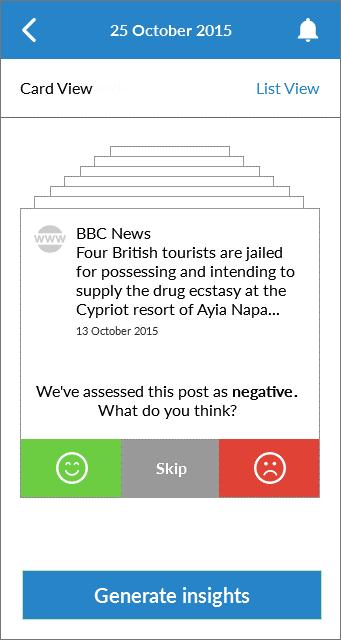
\includegraphics[width=4.2cm]{inc/ui_takedown_step1.jpg}
    \caption{Takedown -- Step 1}
    \label{fig:ui_takedown_step1}
  \end{minipage}
  \begin{minipage}{4.6cm}
    \centering
    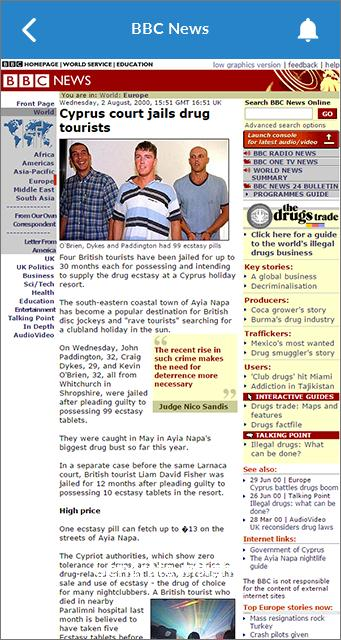
\includegraphics[width=4.2cm]{inc/ui_takedown_step2.jpg}
    \caption{Takedown -- Step 2}
    \label{fig:ui_takedown_step2}
  \end{minipage}
  \begin{minipage}{4.6cm}
    \centering
    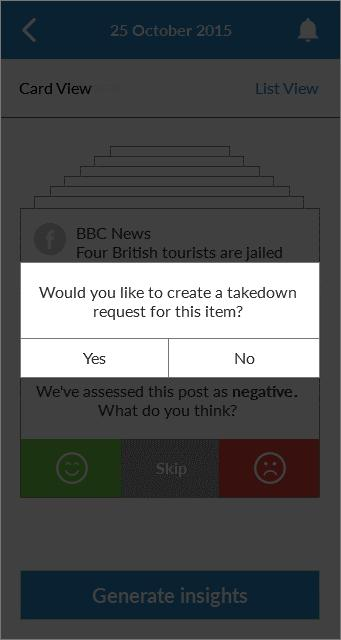
\includegraphics[width=4.2cm]{inc/ui_takedown_step3.jpg}
    \caption{Takedown -- Step 3}
    \label{fig:ui_takedown_step3}
  \end{minipage}
\end{figure}

\begin{minipage}{\textwidth}
  \centering
  \begin{minipage}[t]{4.6cm}
    \vspace{0pt}
    \centering
    \begin{minipage}{4.4cm}
      If the user wants to access additional detail on a post, they need to ``long press'' the card.
    \end{minipage}
  \end{minipage}
  \begin{minipage}[t]{4.6cm}
    \vspace{0pt}
    \centering
    \begin{minipage}{4.4cm}
      Long pressing a post related to a web link opens up a new screen with the article in full view.
    \end{minipage}
  \end{minipage}
  \begin{minipage}[t]{4.6cm}
    \vspace{0pt}
    \centering
    \begin{minipage}{4.4cm}
      If the user wants to create a takedown request, then they need to press the red ``sad face''.
    \end{minipage}
  \end{minipage}
\end{minipage}

\begin{figure}
  \subfigures
  \centering
  \begin{minipage}{4.6cm}
    \centering
    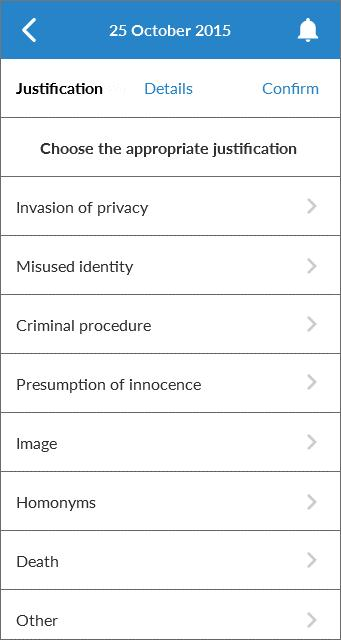
\includegraphics[width=4.2cm]{inc/ui_takedown_step4.jpg}
    \caption{Takedown -- Step 4}
    \label{fig:ui_takedown_step4}
  \end{minipage}
  \begin{minipage}{4.6cm}
    \centering
    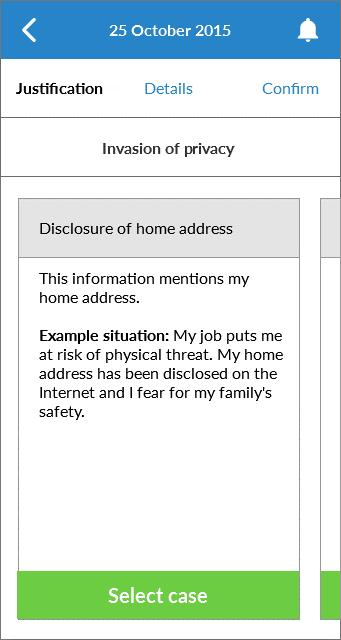
\includegraphics[width=4.2cm]{inc/ui_takedown_step5.jpg}
    \caption{Takedown -- Step 5}
    \label{fig:ui_takedown_step5}
  \end{minipage}
  \begin{minipage}{4.6cm}
    \centering
    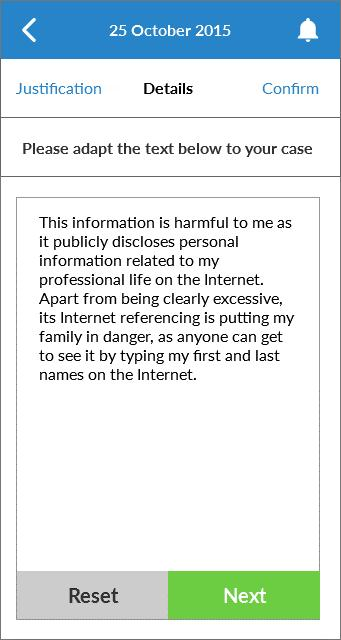
\includegraphics[width=4.2cm]{inc/ui_takedown_step6.jpg}
    \caption{Takedown -- Step 6}
    \label{fig:ui_takedown_step6}
  \end{minipage}
\end{figure}

\begin{minipage}{\textwidth}
  \centering
  \begin{minipage}[t]{4.6cm}
    \vspace{0pt}
    \centering
    \begin{minipage}{4.4cm}
      The user must then select a justification category for the takedown request. It is important that it complements the content of the referenced article.
    \end{minipage}
  \end{minipage}
  \begin{minipage}[t]{4.6cm}
    \vspace{0pt}
    \centering
    \begin{minipage}{4.4cm}
      Each category has a number of subcategories which help the user find an appropriate case that complements the content of the referenced article.
    \end{minipage}
  \end{minipage}
  \begin{minipage}[t]{4.6cm}
    \vspace{0pt}
    \centering
    \begin{minipage}{4.4cm}
      After a case has been selected, the user is provided with sample text that will be placed in the takedown request to supplement the claim.
    \end{minipage}
  \end{minipage}
\end{minipage}

\begin{figure}
  \subfigures
  \centering
  \begin{minipage}{4.6cm}
    \centering
    \includegraphics[width=4.2cm]{inc/ui_takedown_step7.jpg}
    \caption{Takedown -- Step 7}
    \label{fig:ui_takedown_step7}
  \end{minipage}
  \begin{minipage}{4.6cm}
    \centering
    \includegraphics[width=4.2cm]{inc/ui_takedown_step8a.jpg}
    \caption{Takedown -- Step 8a}
    \label{fig:ui_takedown_step8a}
  \end{minipage}
  \begin{minipage}{4.6cm}
    \centering
    \includegraphics[width=4.2cm]{inc/ui_takedown_step8b.jpg}
    \caption{Takedown -- Step 8b}
    \label{fig:ui_takedown_step8b}
  \end{minipage}
\end{figure}

\begin{minipage}{\textwidth}
  \centering
  \begin{minipage}[t]{4.6cm}
    \vspace{0pt}
    \centering
    \begin{minipage}{4.4cm}
      The user can either delegate the job of submitting the request to the app or decide to do it themselves.
    \end{minipage}
  \end{minipage}
  \begin{minipage}[t]{4.6cm}
    \vspace{0pt}
    \centering
    \begin{minipage}{4.4cm}
      If the user opts to do it themselves, then they are emailed a guide on how to complete the request.
    \end{minipage}
  \end{minipage}
  \begin{minipage}[t]{4.6cm}
    \vspace{0pt}
    \centering
    \begin{minipage}{4.4cm}
      If the user delegates the task to the app, they will need to upload a photo that proves their identity.
    \end{minipage}
  \end{minipage}
\end{minipage}

\begin{figure}
  \subfigures
  \centering
  \begin{minipage}{4.6cm}
    \centering
    \includegraphics[width=4.2cm]{inc/ui_takedown_step9.jpg}
    \caption{Takedown -- Step 9}
    \label{fig:ui_takedown_step9}
  \end{minipage}
  \begin{minipage}{4.6cm}
    \centering
    \includegraphics[width=4.2cm]{inc/ui_takedown_step10.jpg}
    \caption{Takedown -- Step 10}
    \label{fig:ui_takedown_step10}
  \end{minipage}
  \begin{minipage}{4.6cm}
    \centering
    \includegraphics[width=4.2cm]{inc/ui_takedown_step11.jpg}
    \caption{Takedown -- Step 11}
    \label{fig:ui_takedown_step11}
  \end{minipage}
\end{figure}

\begin{minipage}{\textwidth}
  \centering
  \begin{minipage}[t]{4.6cm}
    \vspace{0pt}
    \centering
    \begin{minipage}{4.4cm}
      The user can either select to take a new photo or select one from their phone's gallery.
    \end{minipage}
  \end{minipage}
  \begin{minipage}[t]{4.6cm}
    \vspace{0pt}
    \centering
    \begin{minipage}{4.4cm}
      In this example, the user has opted to take a photo of their passport document.
    \end{minipage}
  \end{minipage}
  \begin{minipage}[t]{4.6cm}
    \vspace{0pt}
    \centering
    \begin{minipage}{4.4cm}
      The user can name the photo so that it can be saved and used in other takedown requests.
    \end{minipage}
  \end{minipage}
\end{minipage}

\clearpage

\begin{figure}
  \subfigures
  \centering
  \begin{minipage}{4.6cm}
    \centering
    \includegraphics[width=4.2cm]{inc/ui_takedown_step12a.jpg}
    \caption{Takedown -- Step 12a}
    \label{fig:ui_takedown_step12a}
  \end{minipage}
  \begin{minipage}{4.6cm}
    \centering
    \includegraphics[width=4.2cm]{inc/ui_takedown_step12b.jpg}
    \caption{Takedown -- Step 12b}
    \label{fig:ui_takedown_step12b}
  \end{minipage}
  \begin{minipage}{4.6cm}
    \centering
    \includegraphics[width=4.2cm]{inc/ui_takedown_step12c.jpg}
    \caption{Takedown -- Step 12c}
    \label{fig:ui_takedown_step12c}
  \end{minipage}
\end{figure}

\begin{minipage}{\textwidth}
  \centering
  \begin{minipage}[t]{4.6cm}
    \vspace{0pt}
    \centering
    \begin{minipage}{4.4cm}
      If necessary, the user can attach one or more documents to the takedown request.
    \end{minipage}
  \end{minipage}
  \begin{minipage}[t]{4.6cm}
    \vspace{0pt}
    \centering
    \begin{minipage}{4.4cm}
      The user can also review their documents. If necessary, documents can be renamed or deleted.
    \end{minipage}
  \end{minipage}
  \begin{minipage}[t]{4.6cm}
    \vspace{0pt}
    \centering
    \begin{minipage}{4.4cm}
      All documents will be encrypted when stored and permanently destroyed when no longer required.
    \end{minipage}
  \end{minipage}
\end{minipage}

\subsection{Add Payment Method}

\begin{figure}
  \subfigures
  \centering
  \begin{minipage}{4.6cm}
    \centering
    \includegraphics[width=4.2cm]{inc/ui_payment_step1.jpg}
    \caption{Add Method -- Step 1}
    \label{fig:ui_payment_step1}
  \end{minipage}
  \begin{minipage}{4.6cm}
    \centering
    \includegraphics[width=4.2cm]{inc/ui_payment_step2.jpg}
    \caption{Add Method -- Step 2}
    \label{fig:ui_payment_step2}
  \end{minipage}
\end{figure}

\begin{minipage}{\textwidth}
  \centering
  \begin{minipage}[t]{4.6cm}
    \vspace{0pt}
    \centering
    \begin{minipage}{4.4cm}
      If the user wants to provide new payment details, then they must press the ``add card'' button.
    \end{minipage}
  \end{minipage}
  \begin{minipage}[t]{4.6cm}
    \vspace{0pt}
    \centering
    \begin{minipage}{4.4cm}
      After filling in the required fields, the user must press on the “save” button.
    \end{minipage}
  \end{minipage}
\end{minipage}

\subsection{Remove Payment Method}

\begin{figure}
  \subfigures
  \centering
  \begin{minipage}{4.6cm}
    \centering
    \includegraphics[width=4.2cm]{inc/ui_payment_rm_step1.jpg}
    \caption{Remove Method -- Step 1}
    \label{fig:ui_payment_rm_step1}
  \end{minipage}
  \begin{minipage}{4.6cm}
    \centering
    \includegraphics[width=4.2cm]{inc/ui_payment_rm_step2.jpg}
    \caption{Remove Method -- Step 2}
    \label{fig:ui_payment_rm_step2}
  \end{minipage}
\end{figure}

\begin{minipage}{\textwidth}
  \centering
  \begin{minipage}[t]{4.6cm}
    \vspace{0pt}
    \centering
    \begin{minipage}{4.4cm}
      If the user wants to remove new payment details, then they must press the ``remove card'' button.
    \end{minipage}
  \end{minipage}
  \begin{minipage}[t]{4.6cm}
    \vspace{0pt}
    \centering
    \begin{minipage}{4.4cm}
      The user is then asked if to confirm whether or not they want to remove the card.
    \end{minipage}
  \end{minipage}
\end{minipage}

\clearpage

\subsection{Make Payment}

\begin{figure}
  \subfigures
  \centering
  \begin{minipage}{4.6cm}
    \centering
    \includegraphics[width=4.2cm]{inc/ui_payment_mk_step1.jpg}
    \caption{Make Payment -- Step 1}
    \label{fig:ui_payment_mk_step1}
  \end{minipage}
  \begin{minipage}{4.6cm}
    \centering
    \includegraphics[width=4.2cm]{inc/ui_payment_mk_step2.jpg}
    \caption{Make Payment -- Step 2}
    \label{fig:ui_payment_mk_step2}
  \end{minipage}
\end{figure}

\begin{minipage}{\textwidth}
  \centering
  \begin{minipage}[t]{4.6cm}
    \vspace{0pt}
    \centering
    \begin{minipage}{4.4cm}
      In order to make a payment for a service, the user must press the ``pay'' button.
    \end{minipage}
  \end{minipage}
  \begin{minipage}[t]{4.6cm}
    \vspace{0pt}
    \centering
    \begin{minipage}{4.4cm}
      Once done, a receipt is sent to the user’s email address as record of payment.
    \end{minipage}
  \end{minipage}
\end{minipage}

\clearpage

\subsection{Generate Insights}

\begin{figure}
  \subfigures
  \centering
  \begin{minipage}{4.6cm}
    \centering
    \includegraphics[width=4.2cm]{inc/ui_insight_step1.jpg}
    \caption{Generate Insights -- Step 1}
    \label{fig:ui_insight_step1}
  \end{minipage}
  \begin{minipage}{4.6cm}
    \centering
    \includegraphics[width=4.2cm]{inc/ui_insight_step2.jpg}
    \caption{Generate Insights -- Step 2}
    \label{fig:ui_insight_step2}
  \end{minipage}
  \begin{minipage}{4.6cm}
    \centering
    \includegraphics[width=4.2cm]{inc/ui_insight_step3.jpg}
    \caption{Generate Insights -- Step 3}
    \label{fig:ui_insight_step3}
  \end{minipage}
\end{figure}

\begin{minipage}{\textwidth}
  \centering
  \begin{minipage}[t]{4.6cm}
    \vspace{0pt}
    \centering
    \begin{minipage}{4.4cm}
      Once a report is collated, it is possible to compile a set of insights based on the data gathered.
    \end{minipage}
  \end{minipage}
  \begin{minipage}[t]{4.6cm}
    \vspace{0pt}
    \centering
    \begin{minipage}{4.4cm}
      After pressing the ``generate insights'' button, a set of insights is compiled for the user.
    \end{minipage}
  \end{minipage}
  \begin{minipage}[t]{4.6cm}
    \vspace{0pt}
    \centering
    \begin{minipage}{4.4cm}
      The app groups the user’s posts to date into three categories and then grades their online profile.
    \end{minipage}
  \end{minipage}
\end{minipage}

\clearpage

\subsection{View Recommendations}

\begin{figure}
  \subfigures
  \centering
  \begin{minipage}{4.6cm}
    \centering
    \includegraphics[width=4.2cm]{inc/ui_recommendation_step1.jpg}
    \caption{View Recommendations -- Step 1}
    \label{fig:ui_recommendation_step1}
  \end{minipage}
  \begin{minipage}{4.6cm}
    \centering
    \includegraphics[width=4.2cm]{inc/ui_recommendation_step2.jpg}
    \caption{View Recommendations -- Step 2}
    \label{fig:ui_recommendation_step2}
  \end{minipage}
  \begin{minipage}{4.6cm}
    \centering
    \includegraphics[width=4.2cm]{inc/ui_recommendation_step3.jpg}
    \caption{View Recommendations -- Step 3}
    \label{fig:ui_recommendation_step3}
  \end{minipage}
\end{figure}

\begin{minipage}{\textwidth}
  \centering
  \begin{minipage}[t]{4.6cm}
    \vspace{0pt}
    \centering
    \begin{minipage}{4.4cm}
      Once the user has acquired a grade for their online profile, they can explore ways to improve it.
    \end{minipage}
  \end{minipage}
  \begin{minipage}[t]{4.6cm}
    \vspace{0pt}
    \centering
    \begin{minipage}{4.4cm}
      After selecting the recommendations tab, the user is given strategies to help boost their grade.
    \end{minipage}
  \end{minipage}
  \begin{minipage}[t]{4.6cm}
    \vspace{0pt}
    \centering
    \begin{minipage}{4.4cm}
      In this case, the user is advised to tweet and is given an overview of popular tweets on a subject.
    \end{minipage}
  \end{minipage}
\end{minipage}
